\section{Anhang}

\begin{figure}[H]
    \centering
    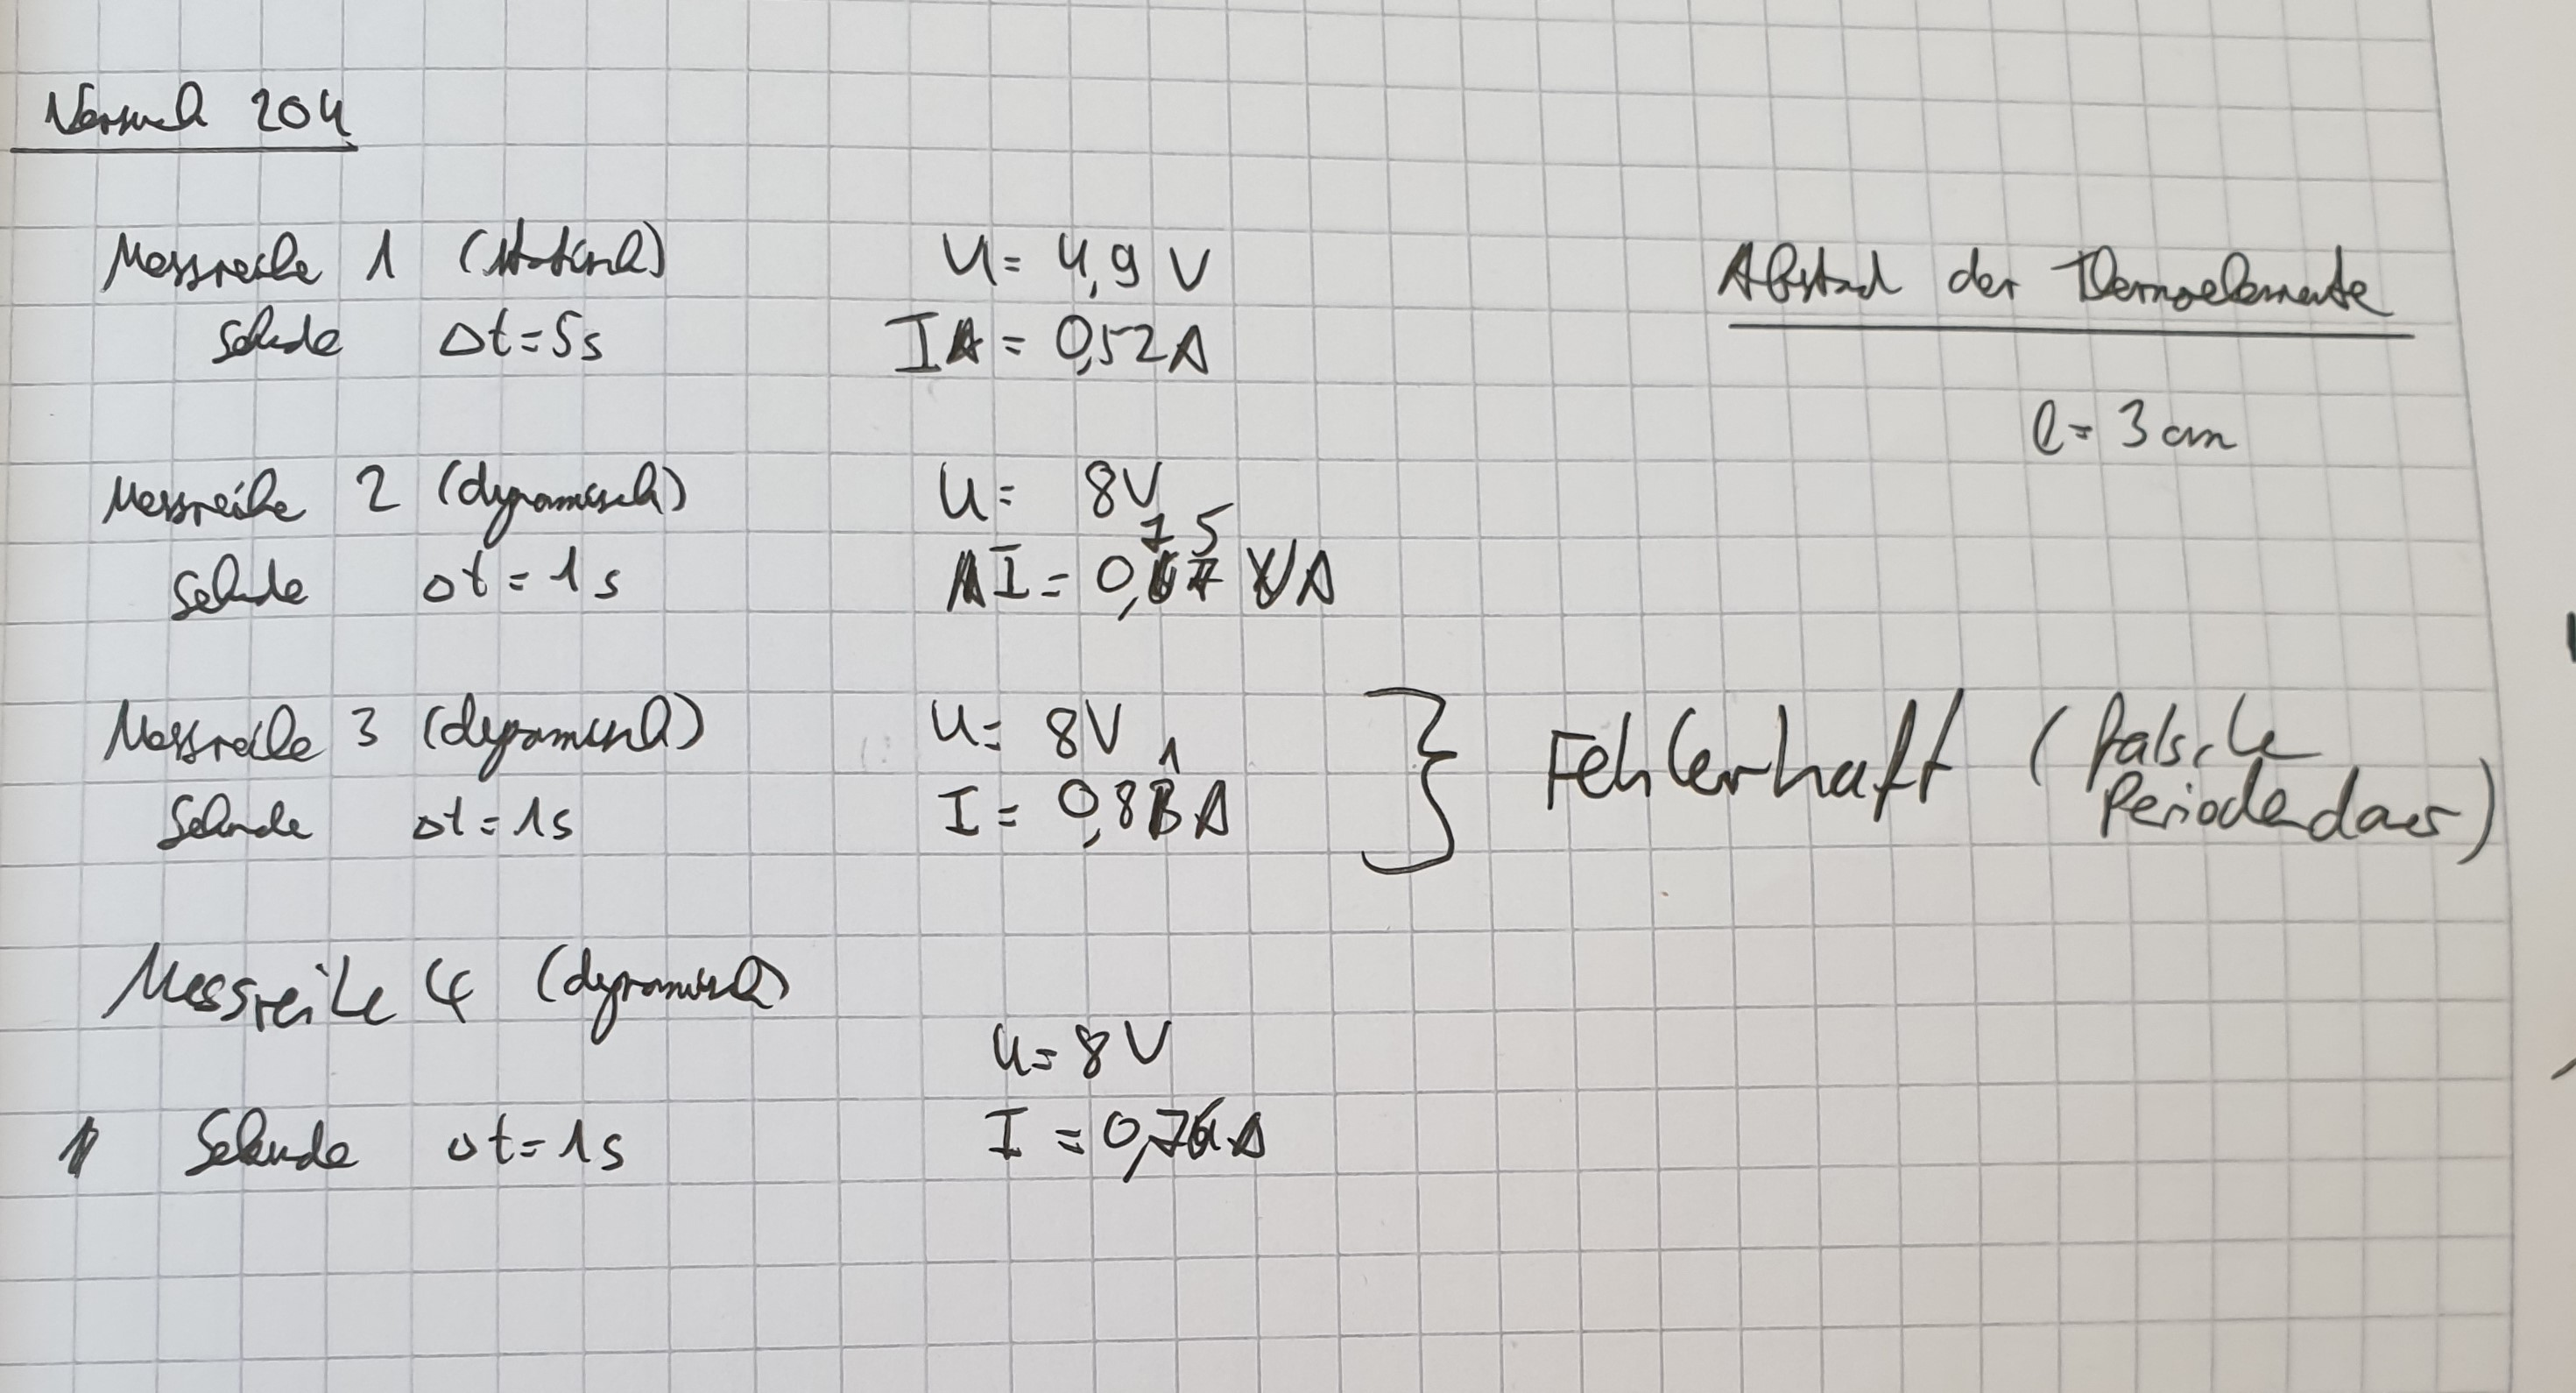
\includegraphics[width=13cm]{content/anhang.jpg}
\end{figure}


%\begin{table}
%     \centering
%          \caption{Erste Messreihe }
%     \csvreader[tabular=c c c c c c c c c c,
%   head=false, 
%   table head= Messung & T1 & T2 & T3 & T4 & T5 & T6 & T7 & T8 & AENDERN\\\midrule,
%    late after line= \\]
%  {content/Data/1_1.csv}{1=\eins, 2=\zwei, 3=\drei, 4=\vier, 5=\fuenf, 6=\sechs, 7=\sieben, 8=\acht, 9=\neun, 10=\zehn}{$\num{\eins}$ & $\num{\zwei}$ & $\num{\drei}$ & $\num{\vier}$ & $\num{\fuenf}$ & $\num{\sechs}$ & $\num{\sieben}$ & $\num{\acht}$ & $\num{\neun}$ & $\num{\zehn}$}
  
%\end{table}

